\documentclass[border=10pt]{standalone}
\usepackage{tikz}
\usepackage{amsmath}
\usetikzlibrary{arrows.meta, positioning, fit, backgrounds, calc}

\begin{document}
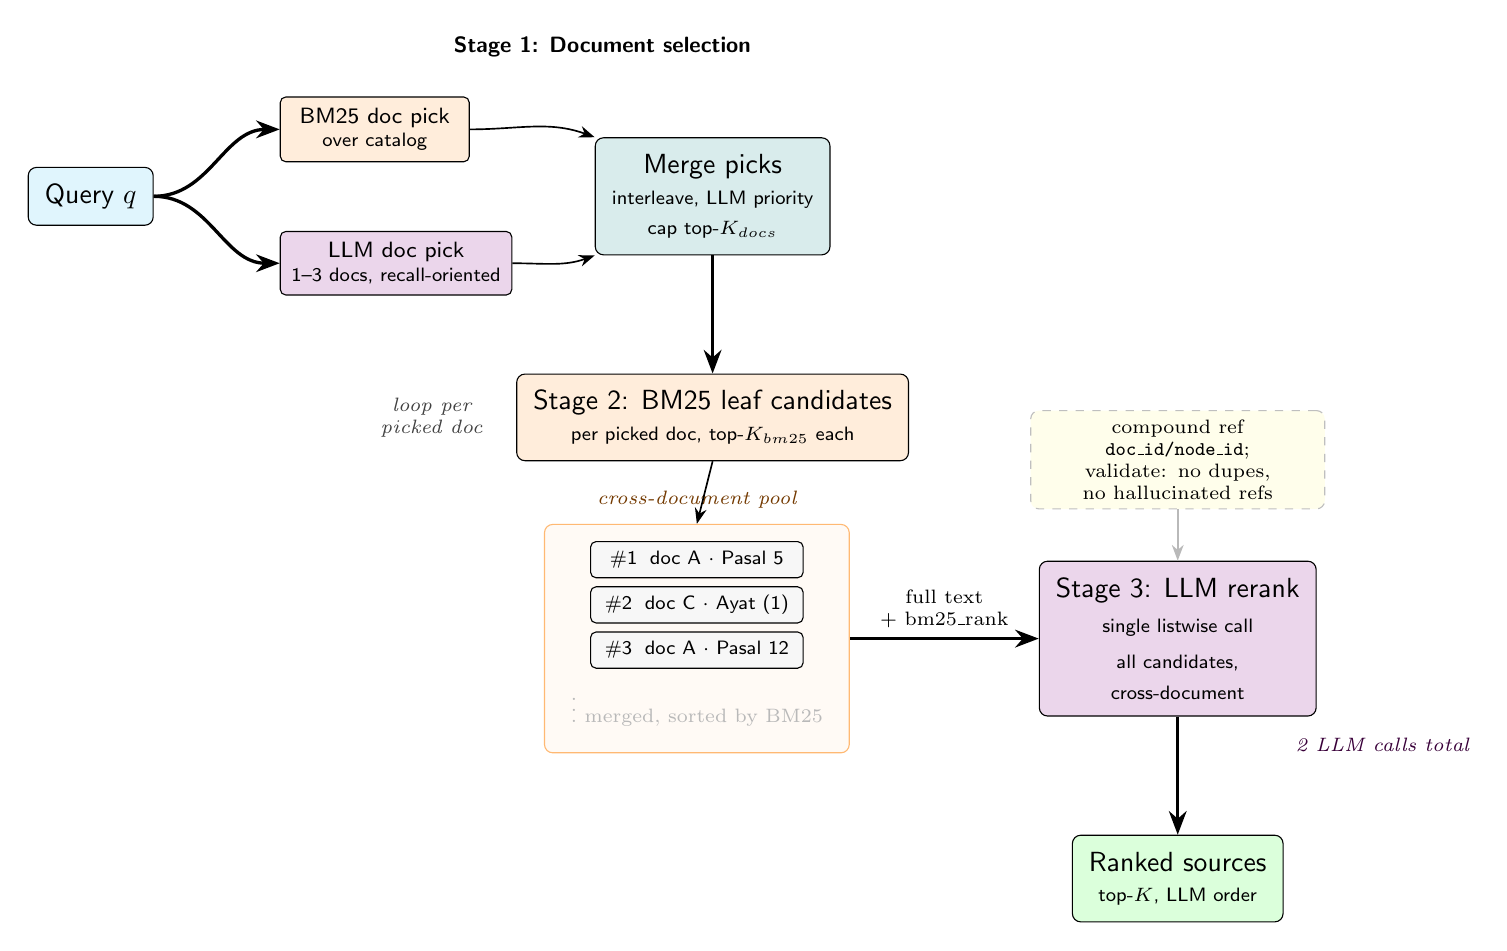
\begin{tikzpicture}[
    font=\small,
    box/.style={draw, rounded corners=3pt, align=center, font=\sffamily,
                inner sep=6pt},
    small/.style={draw, rounded corners=2pt, align=center, font=\footnotesize\sffamily,
                  inner sep=4pt, minimum width=2.4cm},
    cand/.style={draw, rounded corners=2pt, minimum width=2.7cm, minimum height=0.46cm,
                 font=\scriptsize\sffamily, align=left, inner sep=3pt, fill=gray!6},
    flow/.style={-{Stealth[length=3mm]}, very thick},
    arr/.style={-{Stealth[length=2mm]}, semithick},
]

    %==================== QUERY ====================
    \node[box, fill=cyan!12] (q) {Query $q$};

    %==================== STAGE 1: DOC SELECTION (BM25 + LLM merge) ====================
    % two parallel pickers
    \node[small, fill=orange!14, right=1.6cm of q, yshift=0.85cm] (docbm25)
        {BM25 doc pick\\[-1pt]{\scriptsize over catalog}};
    \node[small, fill=violet!16, right=1.6cm of q, yshift=-0.85cm] (docllm)
        {LLM doc pick\\[-1pt]{\scriptsize 1--3 docs, recall-oriented}};

    \draw[flow] (q.east) to[out=0, in=180] (docbm25.west);
    \draw[flow] (q.east) to[out=0, in=180] (docllm.west);

    % merge node
    \node[box, fill=teal!15, right=1.6cm of q, xshift=4.0cm, align=center] (merge)
        {Merge picks\\[-1pt]{\scriptsize interleave, LLM priority}\\[-1pt]
         {\scriptsize cap top-$K_{docs}$}};
    \draw[arr] (docbm25.east) to[out=0, in=160] (merge.north west);
    \draw[arr] (docllm.east) to[out=0, in=200] (merge.south west);

    \node[font=\sffamily\bfseries\footnotesize, above=0.9cm of merge, xshift=-1.4cm]
        {Stage 1: Document selection};

    %==================== STAGE 2: per-doc BM25 candidates ====================
    \node[box, fill=orange!14, below=1.5cm of merge, align=center] (nodebm25)
        {Stage 2: BM25 leaf candidates\\[-1pt]{\scriptsize per picked doc, top-$K_{bm25}$ each}};
    \draw[flow] (merge.south) -- (nodebm25.north);

    \node[font=\scriptsize\itshape, text=gray!50!black, left=0.3cm of nodebm25, align=center]
        {loop per\\ picked doc};

    %==================== merged cross-doc candidate pool ====================
    \node[cand] (c1) at ($(nodebm25.south)+(-0.2,-1.25)$) {\#1\; doc A $\cdot$ Pasal 5};
    \node[cand, below=0.1cm of c1] (c2) {\#2\; doc C $\cdot$ Ayat (1)};
    \node[cand, below=0.1cm of c2] (c3) {\#3\; doc A $\cdot$ Pasal 12};
    \node[font=\scriptsize, text=gray!55, below=0.04cm of c3] (cdots)
        {$\vdots$ merged, sorted by BM25};

    \begin{scope}[on background layer]
        \node[draw=orange!55, rounded corners=3pt, fill=orange!4,
              fit=(c1)(cdots), inner sep=6pt] (candbox) {};
    \end{scope}
    \node[font=\scriptsize\itshape, text=orange!45!black, anchor=south]
        at ([yshift=2pt]candbox.north) {cross-document pool};
    \draw[arr] (nodebm25.south) -- (candbox.north);

    %==================== STAGE 3: LLM listwise rerank ====================
    \node[box, fill=violet!16, right=2.4cm of candbox, align=center, minimum height=1.7cm]
        (rerank) {Stage 3: LLM rerank\\[1pt]{\scriptsize single listwise call}\\[1pt]
                  {\scriptsize all candidates,}\\[-1pt]{\scriptsize cross-document}};
    \draw[flow] (candbox.east) -- node[above, font=\scriptsize, align=center]
        {full text\\ $+$ bm25\_rank} (rerank.west);

    %==================== validation note ====================
    \node[draw=gray!50, dashed, rounded corners=3pt, fill=yellow!8, font=\scriptsize,
          align=center, above=0.65cm of rerank, text width=3.5cm] (note)
        {compound ref \texttt{doc\_id/node\_id};\\
         validate: no dupes,\\ no hallucinated refs};
    \draw[arr, gray!55] (note.south) -- (rerank.north);

    %==================== OUTPUT ====================
    \node[box, fill=green!14, below=1.5cm of rerank, align=center] (out)
        {Ranked sources\\[-1pt]{\scriptsize top-$K$, LLM order}};
    \draw[flow] (rerank.south) -- (out.north);

    %==================== total LLM call emphasis ====================
    \node[font=\scriptsize\itshape, text=violet!45!black, below=0.15cm of rerank, xshift=2.6cm]
        {2 LLM calls total};

\end{tikzpicture}
\end{document}